\documentclass{sig-alternate}
\usepackage{breqn}
\usepackage{pbox}
\usepackage{enumitem, array}
\usepackage{hyperref}
\usepackage{times}
\usepackage{balance}
\usepackage{xspace}
\usepackage{url}
\usepackage{cite}

\setlist{nolistsep}
\setlength{\textfloatsep}{10pt}


\usepackage{listings}
\lstset{
  breaklines=true,
}

% Markup macros for proof-reading
\usepackage[normalem]{ulem} % for \sout
\usepackage{xcolor}
\newcommand{\ra}{$\rightarrow$}
\newcommand{\ugh}[1]{\textcolor{red}{\uwave{#1}}} % please rephrase
\newcommand{\ins}[1]{\textcolor{blue}{\uline{#1}}} % please insert
\newcommand{\del}[1]{\textcolor{red}{\sout{#1}}} % please delete
\newcommand{\chg}[2]{\textcolor{red}{\sout{#1}}{\ra}\textcolor{blue}{\uline{#2}}} % please change

% Put edit comments in a really ugly standout display
\usepackage{ifthen}
\usepackage{amssymb}
\newboolean{showcomments}
\setboolean{showcomments}{true} % toggle to show or hide comments
\ifthenelse{\boolean{showcomments}}
  {\newcommand{\nb}[2]{
    \fcolorbox{gray}{yellow}{\bfseries\sffamily\scriptsize#1}
    {\sf\small$\blacktriangleright$\textit{#2}$\blacktriangleleft$}
   }
   \newcommand{\version}{\emph{\scriptsize$-$working$-$}}
  }
  {\newcommand{\nb}[2]{}
   \newcommand{\version}{}
  }

\newcommand\gs[1]{\nb{Georgios}{#1}}
\newcommand\bv[1]{\nb{Bogdan}{#1}}
\newcommand\as[1]{\nb{Alexander}{#1}}


\newcommand{\inlinecode}[1] {\lstinline[basicstyle=\ttfamily]{#1}}
\newcommand{\f}[2]{\text{\textit{#1}}\mbox{#2}}
\newcolumntype{P}[1]{>{\raggedright\arraybackslash}p{#1}}

\def\sharedaffiliation{\end{tabular}\newline\begin{tabular}{c}}


\newcommand{\ght}{\textsc{GHT}orrent\xspace}
\newcommand{\api}{\textsc{api}\xspace}
\newcommand{\gh}{\textsc{GitHub}\xspace}

\def\tud{\textsuperscript{*}}
\def\tue{\textsuperscript{\dag}}

\usepackage{tikz}
\newcommand*\circled[1]{\tikz[baseline=(char.base)]{
            \node[shape=circle,draw,inner sep=1pt] (char) {#1};}}


\widowpenalty=30000
\clubpenalty=30000


\begin{document}

% --- Author Metadata here ---
%\conferenceinfo{The 11th Working Conference on Mining Software Repositories}{'14 Hyderabad, India}
%\CopyrightYear{2007} % Allows default copyright year (20XX) to be over-ridden - IF NEED BE.
%\crdata{0-12345-67-8/90/01}  % Allows default copyright data (0-89791-88-6/97/05) to be over-ridden - IF NEED BE.
% --- End of Author Metadata ---

\title{Lean GHTorrent: GitHub data on demand}


\numberofauthors{1}

\author{
Georgios Gousios\tud, Bogdan Vasilescu\tue, Alexander Serebrenik\tue, Andy Zaidman\tud\\
\sharedaffiliation
  \begin{tabular}{ccc}
    \affaddr{\tud Delft University of Technology} && \affaddr{\tue Eindhoven University of Technology}\\
   \affaddr{Delft, The Netherlands} && \affaddr{Eindhoven, The Netherlands}\\
   \email{\{g.gousios, a.e.zaidman\}@tudelft.nl} && \email{\{b.n.vasilescu, a.serebrenik\}@tue.nl} \\
  \end{tabular}
}



\maketitle
\begin{abstract}

In recent years, \gh has become the largest code host in the world, with more than 5M developers
collaborating across 10M repositories.
Numerous popular open source projects (such as Ruby on Rails, Homebrew, Bootstrap, Django or JQuery) 
have chosen \gh as their host and have migrated their code base to it.
\gh offers a tremendous research potential. 
For instance, it is a flagship for current open source development, a place for developers to showcase 
their expertise to peers or potential recruiters, and the platform where social coding features or 
pull requests emerged.
However, \gh data is, to date, largely underexplored.
To facilitate studies of \gh, we have created \ght, a scalable, queriable, offline mirror of the data offered 
through the \gh REST API.
In this paper we present a novel feature of \ght designed to offer customisable data dumps on demand.
The new \ght data-on-demand service offers users the possibility to request via a web form 
up-to-date \ght data dumps for any collection of \gh repositories.
We hope that by offering customisable \ght data dumps we will not only lower the ``barrier for entry'' 
even further for researchers interested in mining \gh data (thus encourage researchers to intensify their 
mining efforts), but also enhance the replicability of \gh studies (since a snapshot of the data on which
the results were obtained can now easily accompany each study).
The service is available at \url{http://ghtorrent.org/lean.html}.
\end{abstract}


%!TEX root = main.tex

\section{Introduction}
\label{sec:intro}

During recent years, \gh (2008) has become the largest code host in the world, with more than 5M developers
collaborating across 10M repositories.
Due to its support for distributed version control (Git) and pull-based development~\cite{barr2012cohesive},
as well as its modern Web UI and focus on social coding~\cite{dabbish2012social}, \gh has surpassed in size
and popularity even much older forges such as Sourceforge (1999).
As a result, numerous projects (especially open source) are migrating their code base to \gh (for instance,
the Google query \emph{migrate to github} returns more than 4M results), which now hosts popular projects
such as Ruby on Rails, Homebrew, Bootstrap, Django or jQuery.

Researchers have quickly jumped on board and have started exploring \gh data.
So far, studies focused on
building language models of source code~\cite{allamanis2013mining},
understanding the effects of branching and pull-based software development~\cite{lee2013git, gousios2014exploratory},
uncovering associations between crowdsourced knowledge and software development~\cite{vasilescu2013stackoverflow},
visualizing collaboration and influence~\cite{heller2011visualizing},
exploring the social network of developers~\cite{thung2013network, schall2013follow, jiang2013understanding},
or investigating how the social nature of \gh impacts collaboration and impression formation~\cite{dabbish2012social, marlow2013impression}
and could be used to improve development practices~\cite{pham2013creating, pham2013building}.
More studies are expected to be published this year, since \gh is the topic of the Mining Challenge
at the 2014 edition of the Working Conference on Mining Software Repositories (MSR).
However, as opposed to Stack Overflow (also 2008), the largest Q\&A site for programming-related questions
and the topic of the Mining Challenge at the 2013 edition of MSR, the richness of \gh data remains
largely underexplored in terms of academic publications~\cite{vasilescu2012meta}.

To facilitate studies of \gh, we have created \ght~\cite{gousios2012ghtorrent}, %, gousios2013ghtorent}, 
a scalable,
queriable, offline mirror of the data offered through the \gh REST API.
\ght data has already been used in empirical studies (e.g., \cite{gousios2014exploratory, squire2014forge,
vasilescu2013stackoverflow}).
%, and a subset of it has been selected as the topic of the Mining Challenge
%at the 2014 edition of the Working Conference on Mining Software Repositories (MSR).
%In response to feedback received from \ght users after its official release~\cite{gousios2013ghtorent},
In this paper we present a novel feature designed to offer customisable data dumps on demand.
The new \ght data-on-demand service offers users the possibility to request via a web form up-to-date \ght
data dumps (in both MySQL and MongoDB formats) for any collection of \gh repositories.

Apart from lowering the ``barrier for entry'' even further for researchers interested in mining \gh data,
this data-on-demand service offers several advantages.
Firstly, while the \ght project already offered data dumps of both its raw data (MongoDB, currently more than 2TB)
and metadata (MySQL, currently more than 20GB), downloading and restoring these dumps can be
very time consuming and might not be necessary if a particular analysis is restricted in scope to say a handful
of ``interesting'' \gh projects (e.g., the Ruby on Rails project, for which separate data sets also started being
collected~\cite{wagstrom2013network}).

\begin{figure*}[t]
\begin{center}
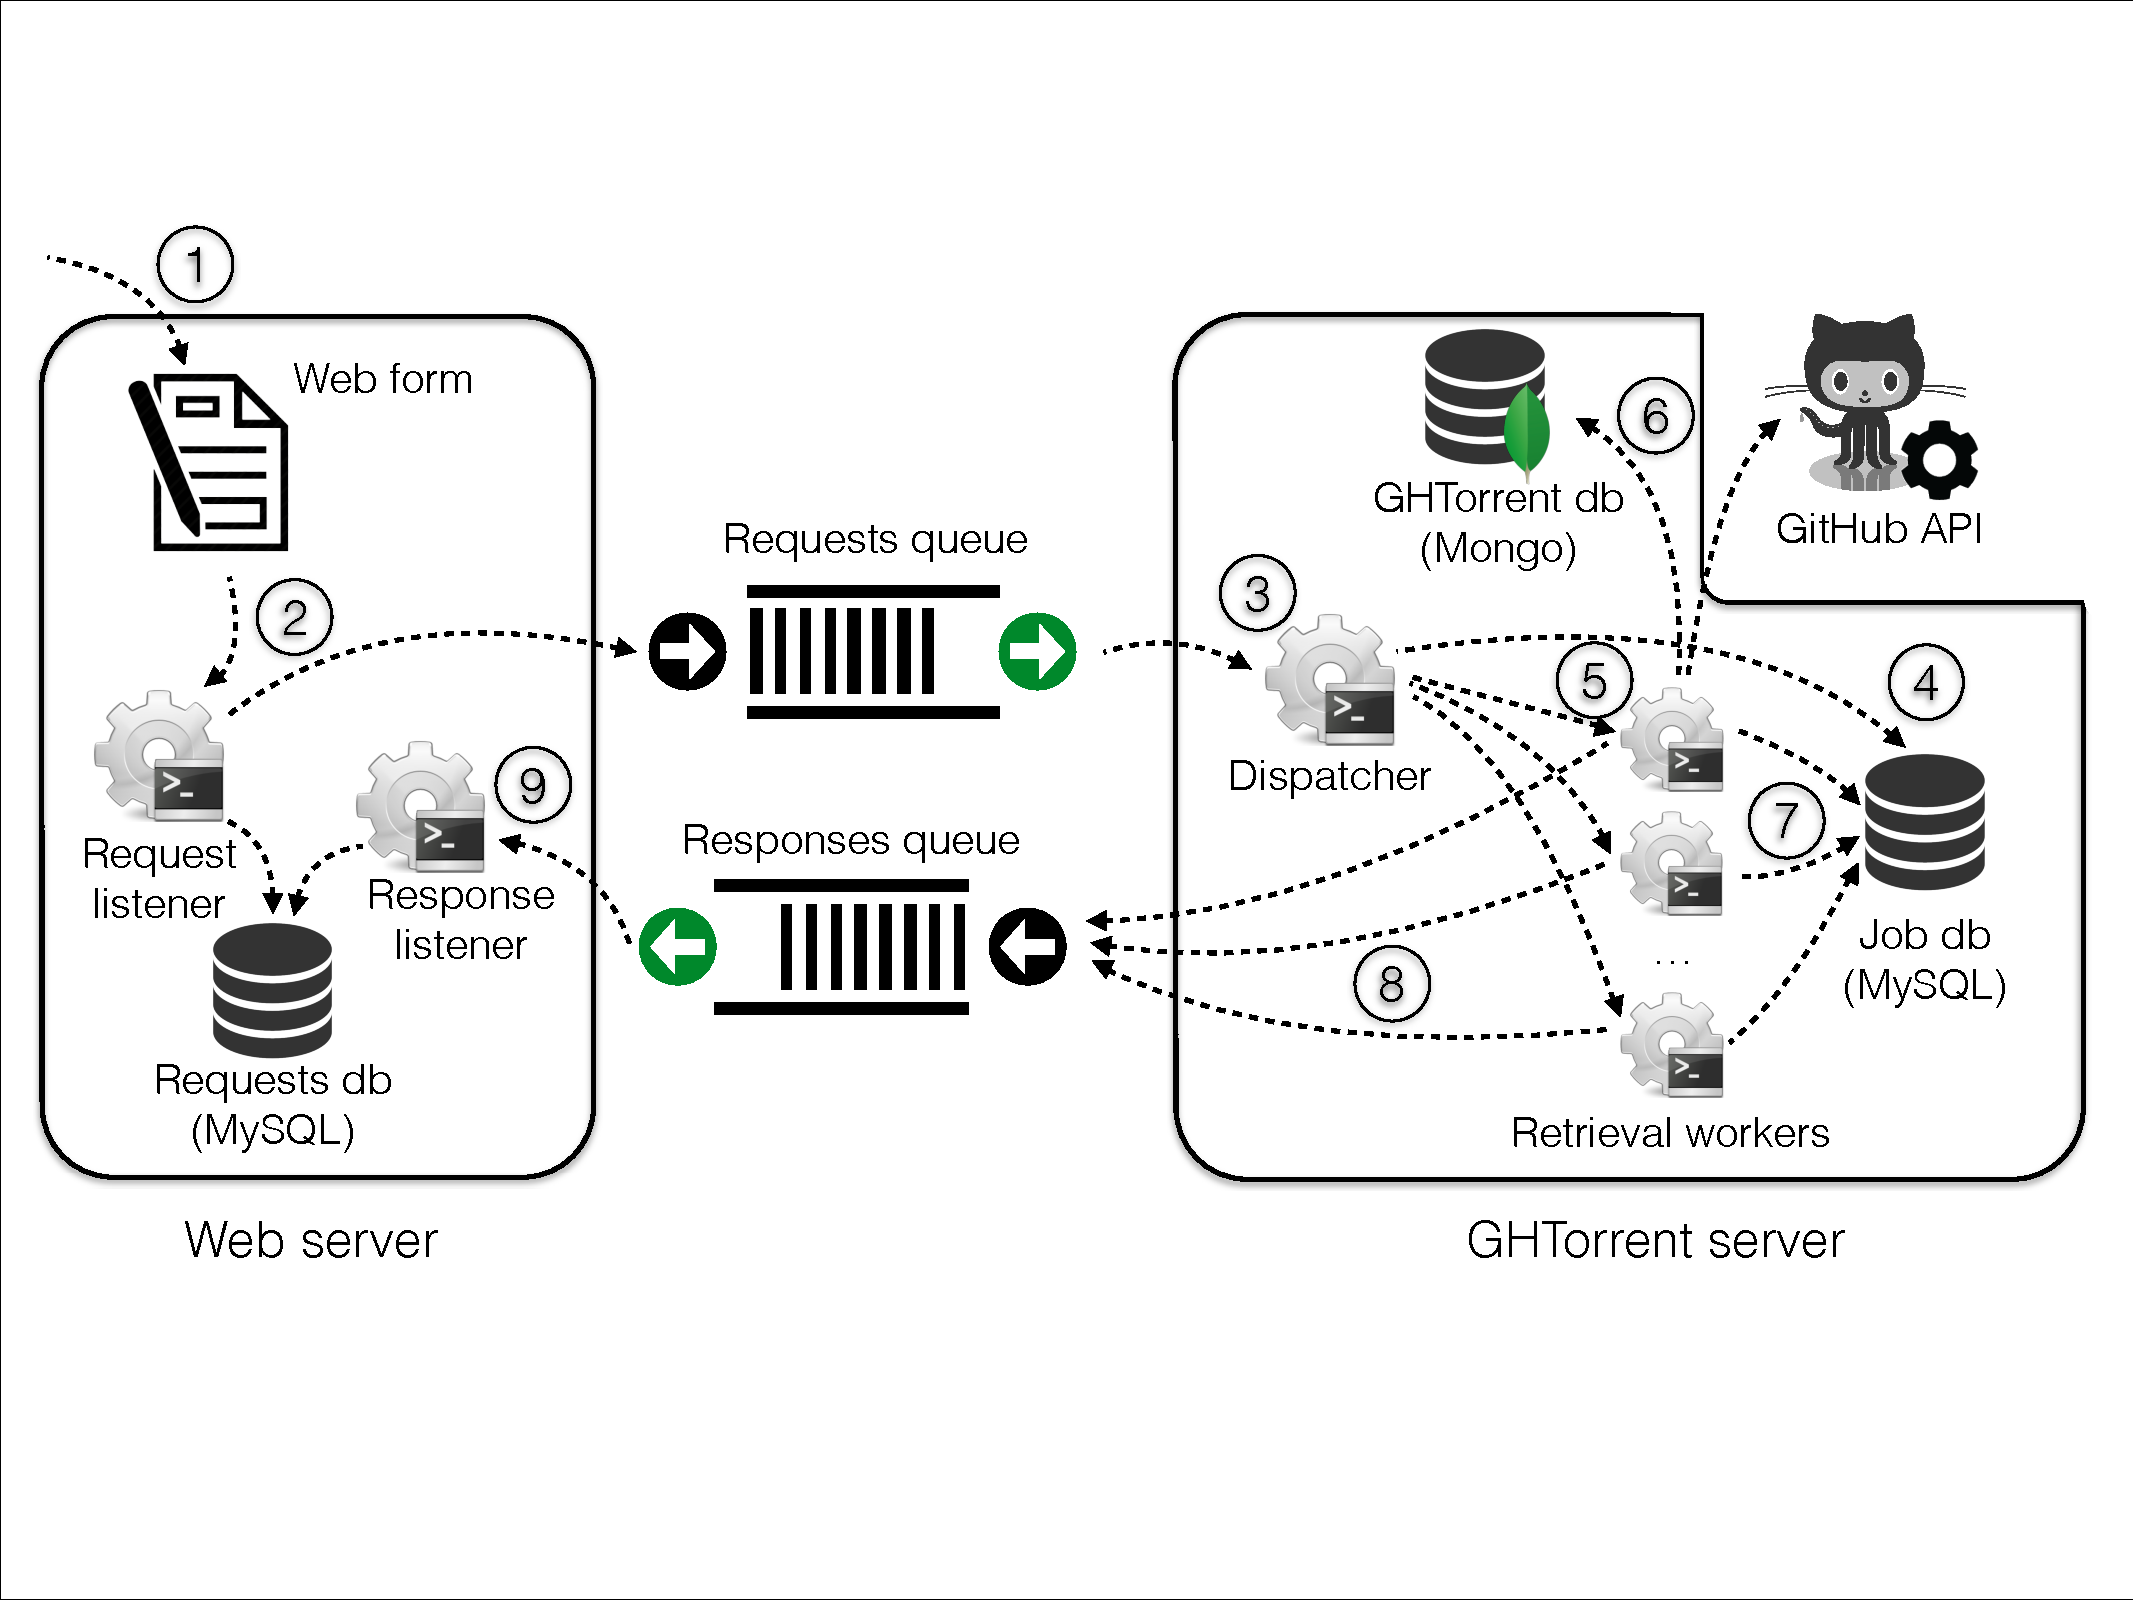
\includegraphics[width=0.8\textwidth, trim=5 160 5 105, clip=True]{figures/architecture.pdf}
\caption{Architecture of the \ght data-on-demand service.}
\label{fig:architecture}
\end{center}
\end{figure*}

Secondly, while the idea of running queries with a restricted scope is not necessarily new with respect to
the official release of \linebreak \ght~\cite{gousios2012ghtorent}, the data-on-demand service enhances replicability
of results obtained using \ght data.
\ght already offered an online query interface with access to an archived version of the relational database,
which could be used to restrict the scope of a query.
However, \gh is a very dynamic platform where developers, projects and wikis are created and deleted constantly.
Therefore, online queries of \ght data may return different results at different times if project data recorded
by \ght has been refreshed in the meantime.
To enhance the replicability~\cite{gonzalez2012reproducibility} of such results, it is therefore preferable to
store the exact snapshot of the data set used in the analysis.

Thirdly, our experiences with curating academic papers based on Stack Exchange data~\cite{vasilescu2012meta}
suggest that researchers prefer to work with data dumps rather than online data explorers
(for reasons such as eliminating the reliance on a third party service, replicability, or integration with existing
tooling or infrastructure).
Even after factoring out papers published at the Mining Challenge of MSR 2013, an overwhelming
fraction of the remaining Stack Exchange papers published after 2010 (when the Stack Exchange data explorer
became available) have used data dumps rather than the data explorer.
We hope that by offering customisable \ght data dumps we will encourage researchers to intensify their efforts
to mine \gh data.

The rest of this paper is organised as follows.
In Section~\ref{sec:arch} we describe the architecture of lean \ght, followed by a discussion of how to use the
service in Section~\ref{sec:usage} and current limitations in Section~\ref{sec:limitations}.
Next, we discuss related work in Section~\ref{sec:relwork}, and present our conclusions in Section~\ref{sec:conclusions}.



%!TEX root = main.tex

\section{Architecture}
\label{sec:arch}

The architecture of the new \ght data-on-demand service consists of two loosely coupled parts:
a web server that handles data requests from users and the \ght server that performs the data extraction.
The two servers communicate via messaging queues.

The interaction between the different subcomponents of the web and \ght servers is illustrated in
Figure~\ref{fig:architecture} and is detailed next.
First, users specify their requests for data by filling in the web form at \url{http://ghtorrent.org/lean.html} \circled{1}.
A request listener validates each request (e.g., it must contain an email address, it must not ask for
more than 100 repositories)\bv{check number}\as{What happens if the limit is exceeded?}
and records metadata about its owner, payload,\as{What kind of payload do you envision and how does the request listener record it?} 
timestamp and status (completed, in progress) in
a relational database.
Then, for each \gh repository part of the request, the listener posts a message to the queue \circled{2}
containing the request identifier, timestamp and repository.

On the \ght server side, a dispatcher listens in on the requests queue \circled{3} and interprets the
messages received as follows.
First, if the message refers to a request for which no previous messages (asking for different repositories)
have been received, a new shared relational database is created to collect metadata for the repositories part
of this request \circled{4}.
This database has the same schema as the original \ght MySQL database~\cite{gousios2013ghtorent},
also described at \url{http://ghtorrent.org/relational.html}.
Then, for each message (repository) referring to the same job, a retrieval worker is instantiated having
as parameters the repository being requested, details for connecting to the job database, and the
timestamp of the request \circled{5}.

Retrieval workers run in parallel and make extensive use of caching.
If the main \ght database already contains data for this repository and this data is not too old
(i.e., the difference between the request timestamp and the timestamp of the last update to this data is at
most three months\bv{check number}), then the shared job database is populated with metadata for this
repository extracted from the main \ght database \circled{6}.\as{Would it be a better strategy to allow the 
user to enforce the database repopulation overwriting the cache? in the same way as with the cached webpages?} 
Otherwise, both the main \ght database and the job database \circled{7} are updated with data freshly extracted
from the \gh API.
This data collection process, again designed as a decentralized process, with decentralization mediated
using a similar \emph{worker queue model}, was described previously~\cite{gousios2013ghtorent}.
Once a retrieval worker finishes, it posts a message to the responses queue \circled{8} signalling
the completion of its task.

On the web server side, a response listener handles incoming response messages (one for each repository
in each request) \circled{9} and updates the status of the job in the requests database.
When ``task complete'' messages have been received for all repositories part of a request, data dumps
are being created from both the job database (MySQL, having the \ght schema~\cite{gousios2013ghtorent})
and the main \ght database (MongoDB, only collections---groupings of MongoDB documents---relevant for this
request are extracted).

Finally, the request owner is notified via email that her job has completed and the requested data dumps
are available for download at a given URL.
\as{This all sounds like a good-weather scenario. Should one describe what happens if something is going wrong? For instance,
how do we ensure consistency of the data or what happens if the mail notification bounces? Do we want some kind of
protection of \ght against malicious bots/users that might try to overload \ght servers?}



%!TEX root = main.tex

\section{Using the service}
\label{sec:usage}
Essentially any study of a restricted collection of \gh repositories can be carried out using the lean \ght offering the advantages of flexibility in selecting the repositories and reproducibility of the results.

We envision, for example, use cases in which researchers interested in mining \gh data start off by using the in-browser
interface to select a number of \gh repositories matching their research goals.
Then, lean \ght can be used to retrieve data for those repositories.

To use the web form at \url{http://ghtorrent.org/lean}, repositories should be input one per line in the dedicated space.
The input format for a repository is \emph{<owner>/<repository>} (for instance, \emph{gousiosg/github-mirror}, or \emph{rails/rails}).

Once a job has been submitted, the user is sent an email with a tracking URL, where information about the status of retrieving
each component (table; commits, forks, pull requests, project members, etc.) of each requested repository is displayed.
Refreshing the tracking page will update the status information.
For example, the following is an excerpt from the tracking page of a request to lean \ght:

[timestamp] WORKING -- Retrieving commits

[timestamp] WORKING -- Retrieving forks

[timestamp] WORKING -- Retrieving pull requests

[timestamp] WORKING -- Retrieving issues

[timestamp] WORKING -- Retrieving project members

[timestamp] WORKING -- Retrieving watchers

[timestamp] WORKING -- Retrieving labels

[timestamp] WORKING -- Retrieving user followers

[timestamp] WORKING -- Retrieving org

[timestamp] FINISHED --
\vspace{0.2cm}

Furthermore, the Ruby scripts provided together with \ght (e.g., scripts to update all the data related to a given repository
or a given user; see the \ght \gh repository \url{https://github.com/gousiosg/github-mirror}) allow users of lean \ght, 
once they restore locally the database dumps they requested, to update their local copies independently.


\as{Would it make sense to mention the SQL-like interface as a front-end? For
instance, if I'm interested in all projects with at least 10 different committers and at least 100 pull requests, I would use this
SQL-like interface to find the repositories, and then provide them to the \ght DOD webform... Or does this reduce the novelty of the approach / require too much work?}


%!TEX root = main.tex

\section{Related work}
\label{sec:relwork}



%!TEX root = main.tex

\section{Conclusions}
\label{sec:conclusions}

We presented a novel feature of \ght that allows users to request \gh data dumps on demand
for any collection of \gh projects (repositories).
Lean \ght offers several advantages, being lightweight and easy to use, fostering replicability
and offering flexibility and independence to researchers interested in mining \gh.
Together with the existing \ght infrastructure, the new lean data-on-demand service lowers 
the ``barrier for entry'' for \gh miners to a minimum.
We hope this will encourage researchers to intensify their efforts to mine \gh data, as well as
serve as inspiration for others willing to share software engineering datasets (the implementations
of both \ght and lean \ght are publicly available).

%In recent years, \gh has become the largest code host in the world, with more than 5M developers
%collaborating across 10M repositories.
%Numerous popular open source projects (such as Ruby on Rails, Homebrew, Bootstrap, Django or JQuery)
%have chosen \gh as their host and have migrated their code base to it.
%\gh offers a tremendous research potential.
%For instance, it is a flagship for current open source development, a place for developers to showcase
%their expertise to peers or potential recruiters, and the platform where social coding features or
%pull requests emerged.
%However, \gh data is, to date, largely underexplored.
%To facilitate studies of \gh, we have created \ght, a scalable, queriable, offline mirror of the data offered
%through the \gh REST API.
%In this paper we present a novel feature of \ght designed to offer customisable data dumps on demand.
%The new \ght data-on-demand service offers users the possibility to request via a web form
%up-to-date \ght data dumps for any collection of \gh repositories.
%We hope that by offering customisable \ght data dumps we will not only lower the ``barrier for entry''
%even further for researchers interested in mining \gh data (thus encourage researchers to intensify their
%mining efforts), but also enhance the replicability of \gh studies (since a snapshot of the data on which
%the results were obtained can now easily accompany each study).
%The service is available at \url{http://ghtorrent.org/lean}.

%!TEX root = main.tex

\paragraph*{Acknowledgements}
\label{sec:acknowledgements}

Georgios Gousios is funded throught the NWO TestRoots project (639.022.314).
Bogdan Vasilescu has been supported by the research project NWO 600.065.120.10N235 financed by Nederlandse Organisatie voor Wetenschappelijk Onderzoek (NWO). 



%{\small
\bibliographystyle{abbrv}
\bibliography{ref}
%}

\end{document}
